\documentclass[12pt,a4paper]{article}
\usepackage{geometry}
\usepackage[numbers]{natbib}
\usepackage{amssymb, amsmath}
\usepackage{graphicx}
\usepackage{grffile}
\graphicspath{{../Figures/}}
\usepackage{gensymb}
\usepackage[font=small]{caption}
\usepackage[utf8]{inputenc}
\usepackage[english]{babel}
\usepackage{fancyhdr}
\usepackage[raggedright]{titlesec}
\usepackage{subcaption}
\usepackage{multirow}
\usepackage{dirtytalk}
\usepackage{framed}
\usepackage[normalem]{ulem}
\usepackage[pdftex,breaklinks]{hyperref}
\hypersetup{
  colorlinks   = true, %Colours links instead of ugly boxes
  urlcolor     = green, %Colour for external hyperlinks
  linkcolor    = blue, %Colour of internal links
  citecolor   = red %Colour of citations
}


\begin{document}
\author{Katrina Ashton}


\pagestyle{fancy}
\fancyhf{}
\rhead{\thepage}
\lhead{u5586882}

\section{What I've done}
\begin{itemize}
  \item Cleaned up my code
  \item Worked on report
  \item Checked if Vicon is causing the poor depth readings (doesn't appear to have any effect).
\end{itemize}

\section{Parts of report to look at}
\begin{itemize}
\item Results (page 38)
\end{itemize}

\section{Questions}
\begin{itemize}
\item Should I get another dataset? If I do I can try to vary the amount of structure and/or texture. The carpet is back so I can use that for more texture (although the samll box also had a lot of texture and is now gone). I'm not sure if I'll have enough space in the report to talk about it though, I'm about at the page limit even though I haven't finished writing up all of the sections.
\item Should I test the algorithms on the external dataset?
\item At this point is it worth trying to get ICP and/or the Photometric error method working? (ICP shouldn't be too difficult using the built-in MATLAB stuff. The photometric error thing will be harder).
\item Do you still want me to have a look at the control data and how it compares to the actual trajectory?
\item Are we going to try anything with closing the loop/other mapping stuff?
\end{itemize}

\section{Comments}
\begin{itemize}
  \item I ended up doing the coordiante transforms before saving the trajectory to avoid vaing to go through each frame to get the proper rotation for every translation.
  \item It doesn't seem like the Vicon is the issue with the depth. My guess is either motion or angle.
  \item I recorded a rosbag looking at how the RealSense deals with angles and distances, but it was too big to fit on my sd card. I'll bring in my external hard-drive and start processing it sometime in the next few days.
\end{itemize}

  \begin{figure}[b!]
    \begin{subfigure}[t]{\textwidth}
    \centering
      \includegraphics[width=80mm, trim = 100 280 100 290, clip]{pc_investigation/MATLAB_a.pdf}
      \caption{Example point cloud taken from RealSense attached to quadcopter}
      \label{f: pcs quad}
    \end{subfigure}  \\
    \begin{subfigure}[t]{0.5\textwidth}
      \includegraphics[width=80mm, trim = 100 300 100 290, clip]{vicon_test/without.pdf}
      \caption{Point cloud taken of scene from still RealSense camera, without Vicon on}
    \end{subfigure} %
    ~
    \begin{subfigure}[t]{0.5\textwidth}
    \centering
      \includegraphics[width=80mm, trim = 100 300 100 290, clip]{vicon_test/with.pdf}
      \caption{Point cloud taken of scene from still RealSense camera, with Vicon on}
    \end{subfigure} 
    \caption{Investigating soures of error in depth measurements via visualizing point clouds. Note that all point clouds have been aligned with the quadcopter-fixed frame.}
    \label{f: pcs}
  \end{figure}

    % \begin{figure}[p]
    %   \begin{subfigure}[t]{0.5\textwidth}
    %   \centering %l b r t
    %     \includegraphics[width=60mm, trim = 20mm 235mm 135mm 10mm, clip]{frames/frames.pdf}
    %     \caption{World frame}
    %   \end{subfigure} %
    %   ~
    %   \begin{subfigure}[t]{0.5\textwidth}
    %   \centering
    %     \includegraphics[width=60mm, trim = 78mm 240mm 78mm 10mm, clip]{frames/frames.pdf}
    %     \caption{Quadcopter world-fixed frame (used in ground truth)}
    %   \end{subfigure} %
    %   \\
    %   \begin{subfigure}[t]{0.5\textwidth}
    %   \centering
    %     \includegraphics[width=60mm, trim = 20mm 235mm 135mm 10mm, clip]{frames/frames.pdf}
    %     \caption{Quadcopter-fixed frame, the (positive) $x$-axis points forward}
    %   \end{subfigure} %
    %   ~
    %   \begin{subfigure}[t]{0.5\textwidth}
    %   \centering
    %     \includegraphics[width=60mm, trim = 135mm 240mm 20mm 10mm, clip]{frames/frames.pdf}
    %     \caption{Camera-fixed frame, the (positive) $z$-axis points forward}
    %   \end{subfigure} %
    %   \\
    %   \begin{subfigure}[t]{\textwidth}
    %   \centering
    %     \includegraphics[width=60mm, trim = 10mm 150mm 125mm 75mm, clip]{frames/frames2.pdf}
    %     \caption{Camera-fixed frame (orange) shown in relation to quadcopter-fixed frame (blue)}
    %     \label{fs: frames c2q}
    %   \end{subfigure}
    %   \caption{3D coordinate frames}
    %   \label{f: frames}
    % \end{figure}

% \newpage
% \begin{figure}[h]
  % \begin{subfigure}[t]{0.5\textwidth}
  % \centering
  %   \includegraphics[width=80mm]{../quad/basic-reg-saves/et_all_40.png}
  %   \caption{Translation error}
  % \end{subfigure} %
%   ~
%   \begin{subfigure}[t]{0.5\textwidth}
%     \includegraphics[width=80mm]{../quad/basic-reg-saves/eR_all_40.png}
%     \caption{Rotation error}
%   \end{subfigure}
%   \caption{Vision error for various registration techniques with 40 frames skipped}
%   \label{f: quad3 error}
% \end{figure}

% \begin{figure}[h]
%   \begin{subfigure}[t]{0.5\textwidth}
%   \centering
%     \includegraphics[width=80mm]{../quad/basic-reg-saves/et_all_30.png}
%     \caption{Translation error}
%   \end{subfigure} %
%   ~
%   \begin{subfigure}[t]{0.5\textwidth}
%     \includegraphics[width=80mm]{../quad/basic-reg-saves/eR_all_30.png}
%     \caption{Rotation error}
%   \end{subfigure}
%   \caption{Vision error for various registration techniques with 30 frames skipped}
%   \label{f: quad3 error 30}
% \end{figure}

% \begin{figure}[p]
% \begin{subfigure}[t]{0.5\textwidth}
%   \centering
%     \includegraphics[width=80mm]{../quad/basic-reg-saves/rtrj_gt_40.png}
%   \caption{Ground truth from Vicon}
%   \end{subfigure}%
%   ~
%   \begin{subfigure}[t]{0.5\textwidth}
%   \centering
%     \includegraphics[width=80mm]{../quad/basic-reg-saves/rtrj_rgb_40.png}
%   \caption{Estimated trajectory for Essential Matrix method, start at origin. Note axes scaling x4}
%   \end{subfigure}
%   \\
%   \begin{subfigure}[t]{0.5\textwidth}
%   \centering
%     \includegraphics[width=80mm]{../quad/basic-reg-saves/rtrj_d_40.png}
%   \caption{Estimated trajectory for Kabsch method, start at origin. Note axes scaling x2}
%   \end{subfigure}%
%   ~
%   \begin{subfigure}[t]{0.5\textwidth}
%   \centering
%     \includegraphics[width=80mm]{../quad/basic-reg-saves/rtrj_pnp_40.png}
%   \caption{Estimated trajectory for PnP method, start at origin. Note axes scaling x2}
%   \end{subfigure}
%   \caption{Trajectory visualizations for third quad dataset}
%   \label{f: quad3 trj}
% \end{figure}

% \begin{figure}[h]
% \begin{subfigure}[t]{\textwidth}
%   \centering
%     \includegraphics[width=80mm]{../quad/basic-reg-saves/rtrj_d_40.png}
%   \caption{RANSAC Kabsch}
%   \end{subfigure}%
%   \\
%   \begin{subfigure}[t]{0.5\textwidth}
%   \centering
%     \includegraphics[width=80mm]{../quad/basic-reg-saves/rtrj_de_40.png}
%   \caption{Kabsch with Essential Matrix inliers}
%   \end{subfigure}%
%   ~
%   \begin{subfigure}[t]{0.5\textwidth}
%   \centering
%     \includegraphics[width=80mm]{../quad/basic-reg-saves/rtrj_dp_40.png}
%   \caption{Kabsch with PnP inliers}
%   \end{subfigure}
%   \caption{Trajectory visualizations for third quad dataset, Kabsch method with different inliers}
%   \label{f: quad3 kabsch}
% \end{figure}





\bibliographystyle{abbrvnat}
\bibliography{../Report/ENGN4217}

\end{document}